\begin{figure}[h]
    \centering 
  \begin{subfigure}[b]{0.5\textwidth}
    \centering
    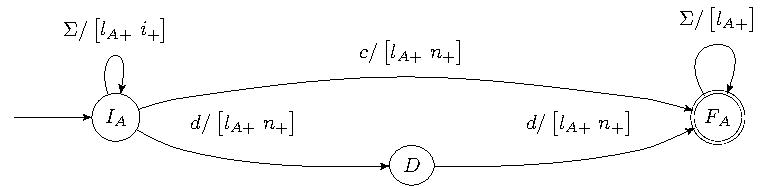
\includegraphics[scale=\autscale]{a}
    \caption{The automaton $A'$, whose Parikh registers count the length of the
    string accepted by the automaton (register $l_A$), the start offset of the
    substring ($i$) and length ($n$) of the substring matching
    $\Regex{c\RegexOr{}dd}$. Note the symbolic transitions in the starting and
    accepting states matching any symbol in the alphabet!}\label{fig:aut_a}
      %\Description[SHORT]{LONG}
  \end{subfigure}
  \begin{subfigure}[b]{0.5\textwidth}
    \centering
    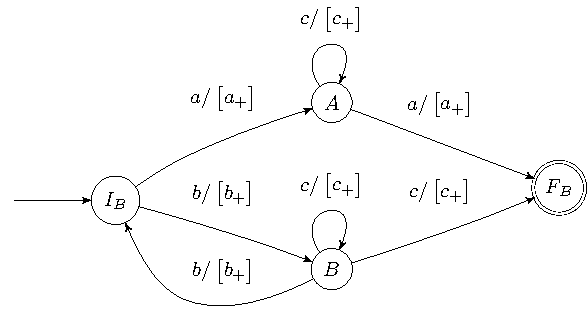
\includegraphics[scale=\autscale]{b}
    \caption{The automaton $B$, where the Parikh registers count the length of
    the string in register $l_B$.}\label{fig:aut_b}
      %\Description[SHORT]{LONG}
  \end{subfigure}
  \caption{The collection of automata we use as running
  examples}\label{fig:examples}
\end{figure}


In this section we will introduce an intuition for how a string constraint
problem in an automata-based solver like \OstrichPlus{} is translated to a
Parikh automata intersection problem and solved using \Calculus{}. First, by a
Parikh automaton we mean a standard non-deterministic finite automaton (NFA)
with a set of integer registers (Parikh registers) that are incremented (or
decremented) at each transition. In the automata of \cref{fig:examples}, we will
use the notation $a / \begin{bmatrix} x_+ \end{bmatrix}$ to mean that a
transition reads an input character $a$ and increments register $x$ by one. We
will omit zero-valued increments and assume that all registers are scoped to
their automaton. The increments are usually represented as a vector (hence the
brackets), but as it is mostly sparse here, we use the symbolic notation
$\begin{bmatrix} x_{1+} \end{bmatrix}$ rather than the more cumbersome $\left[
0, 1,  0 , \ldots, 0 \right]$.

Note that the labels of transitions can be ranges of characters with $\Sigma$
representing any character in the alphabet.

We use PCRE regular expression notation here and throughout the paper, writing
them $\Regex{\texttt{like this}}$. This means that $\RegexOr{}$ is alternation,
$\mathtt{*}$ the Kleene star, and $\mathtt{.}$, matches any single character.

For the length of a string $s$, we write $\Length{s}$.

\begin{example}\label{ex:string-constraints} Consider the following set of
    string constraints:
\begin{constraints}
    \item\label{const:s1-in-c-dd} $s_1 \in \Language(\Regex{c\RegexOr{}dd})$.
    \item\label{const:s2-in-b} $s_2 \in \Language(B)$, the language accepted by
    automaton~$B$ of \cref{fig:aut_b}.
    \item\label{const:s1-substring} $s_1 = \Substring(s_2, i, n)$, that is $s_1$ is an
    $n$-length substring of $s_2$ starting at offset $i$.
    \item\label{const:more-inside-than-before} $n > i$, that is what comes
    before $s_1$ in $s_2$ is shorter than $s_1$.
    \item\label{const:something-before-and-after} $i > 0 \land \Length{s_2} -i -n > 0$, that
    is there is at least one character in $s_2$ after $s_1$.
\end{constraints}
\end{example}

To solve \cref{ex:string-constraints} using \Calculus{} in a theorem proving
context, \cref{const:s1-in-c-dd,const:s2-in-b,const:s1-substring} can be
translated to the product of Parikh automata $B \times A'$, where $A'$
(\cref{fig:aut_a}) is the Parikh automata obtained by applying the encoding of
$\Substring$ described in \cite{ostrich-plus}. That description can then be used
to obtain values for the subsstring offsets $i, n$.

Intuitively, \cref{ex:string-constraints} are unsatisfiable. By inspecting the
automata, we realise that the path using $\Char{dd}$ in $A'$ is unusable since
are no $\Char{d}$-labelled transitions in $B$. This means that $s_1 = \Char{c}$,
and thus $n = 1$. That means that \cref{const:more-inside-than-before} implies
that $i = 0$. However, no path through $B$ passes by a $\Char{c}$ without a
preceding character. Therefore, already
\cref{const:s1-in-c-dd,const:s1-in-c-dd,const:s1-substring,const:more-inside-than-before}
together are unsatisfiable.


Our approach to the computation of the Parikh image (and therefore the solution
to the intersection problem posed by \cref{ex:string-constraints}) consists of
two applications of laziness; late computation of products of automata, and lazy
enforcement of connectivity constraints. Both are in contrast to the eager
approach to finding the Parikh image described in~\cite{generate-parikh-image},
that would have started by computing the product $A' \times B$, translated it to
a Presburger formula with $i, n$ etc as free variables, and then plugged in
\cref{const:more-inside-than-before,const:something-before-and-after}.

Starting with an interactive theorem prover and the goal of solving the Parikh
automata intersection problem, we associate each transition $\Transition$ of
$A'$ and $B$ with a fresh nonnegative integer variable from,
$\TransitionVar_\Transition$, identically to \cite{generate-parikh-image}. These
variables represent how many times each transition is taken. Hence, the final
counter value for counters $r_1, \ldots, r_k$ of each automaton is the
element-wise sum:
\begin{equation}\label{eq:counter-sums}
\begin{bmatrix} 
  r_1 \\
  \vdots\\
  r_k \\
\end{bmatrix} = \sum_\Transition \TransitionVar_\Transition \cdot 
  \IncrementVec_\Transition \text{ where $\IncrementVec_\Transition$ are the increments of transition $\Transition$}.
\end{equation}

\begin{figure}[h]
    \centering 
  \begin{subfigure}[b]{0.5\textwidth}
    \centering
    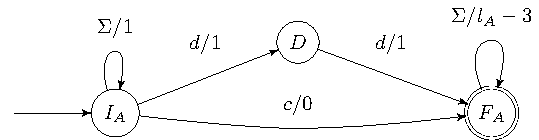
\includegraphics[scale=\autscale]{a_annotated}
    \caption{ $A'$ with its associated transition variables in symbolic form.
    Note: unused ($0$) self-loops at $I_{A'}$ and $F_{A'}$ have been pruned for
    readability.}\label{fig:aut_a_annotated}
      %\Description[SHORT]{LONG}
  \end{subfigure}
  \begin{subfigure}[b]{0.5\textwidth}
    \centering
    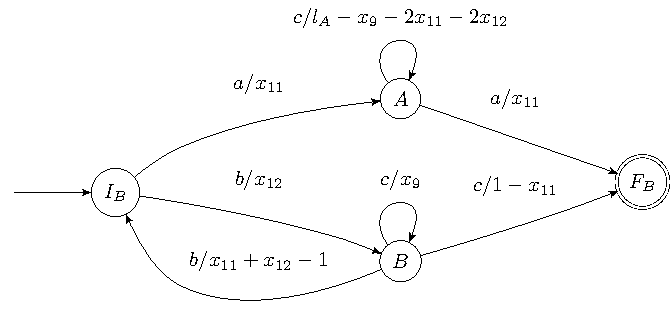
\includegraphics[scale=\autscale]{b_annotated}
    \caption{$B$ with its associated transition variables in symbolic forms.
    Note that state $B$ is now completely dead.}\label{fig:aut_b_annotated}
      %\Description[SHORT]{LONG}
  \end{subfigure}
  \caption{The starting automata, without their counter increments and with
  their transition variables in symbolic form.}\label{fig:propagated}
\end{figure}


We proceed by adding linear constraints requiring transition variables to
represent a flow through their automaton by adding linear constraints stating
that the number of incoming transitions is equal to the number of outgoing ones.
E.g. state $B$ would have the sum $\cancel{x_{\Tuple{B, \Char{c}, B}}} +
x_{\Tuple{I_B, \Char{b}, B}} = \cancel{x_{\Tuple{B, \Char{c}, B}}}  +
x_{\Tuple{B, \Char{c}, F_B}} + x_{\Tuple{B, \Char{b}, I_B}}$ where we let
$x_{\Tuple{q, l, c'}}$ refer to the integer variable associated with a
transition from state $q$ to state $q'$ with label $l$. Note that the self-loop
cancels itself out. This means that for automata where a loop can become
unreachable, additional constraints would be required to ensure reachability.
However, being lazy, we put off that work until later.

Performing symbolic reasoning on these equations and plugging the corresponding
symbolic representation of the constraints on each corresponding integer
variable back as an annotation on its transition, we obtain the two automata in
\cref{fig:propagated}.

Several transitions are already marked as unuseable (have a transition variable
value of $0$) or always present (have a transition variable with a constant
value greater than zero) by just applying standard linear equation solving to
the flow equations described above. Note that this includes
\cref{const:more-inside-than-before,const:something-before-and-after}, which are
related to the transition variables through the sums described in
\cref{eq:counter-sums}. This means that we effectively can prune $A'$ of its
upper path when continuing the proof, as it is incongruent with the flow
equations and \cref{ex:string-constraints}. Note that the per-automata length
counting registers have been assigned the same solver variable $l_A$. Since they
have to be equal, either one can be used in both automata.

Notably, one such conclusion is that $i > 0$ from
\cref{const:something-before-and-after}. From flow preservation we have that the
$F_{A'}$ to $F_{A'}$ transition is represented by $l_A - n - i$.
\footnote{Intuitively, the total length is made up of what is before, inside and
after the substring.} This in turn through \cref{const:more-inside-than-before}
forces $n \geq 2$, which in turn (through flow-preservation) forces a path from
$I_{A'}$ to $F_{A'}$ through $D$, rather than the single-transition path from
$I_{A'}$ to $F_{A'}$. This immediately implies that the problem is
unsatisfiable, since we know this transition has no correspondance in automaton
$B$. 

However, \Calculus{} does not at this point, and we press on with concluding
that none of the loops of $A'$ at this stage can become disconnected since
they are at the initial and final states, both of which are trivially reachable
for any assignments of the non-constant transition variables. This means that
all valid counter assignments of $A'$ are described by \cref{eq:counter-sums}
and the flow equations alone without the need for expensive connectivity
constraints.

After concluding this, we have a choice of two paths through automaton $B$; the
upper through state $A$ or the lower through state $B$. We case split on a
problem-aware basis by selecting a transition variable that would disconnect
some strongly connected component of automaton $B$, in this case the transition
form $I_B$ to state $B$. We divide it into the cases used ($> 0$) or unused ($ =
0$) since those are the threshold values of the calculus, preferring the latter
option on the first-fail principle.

At this point we have two small, stick-like automata after discounting all
transitions with a corresponding transition variable that is zero, and can try
to compute their product. Doing so, we will immediately notice that the
$\Char{d}$-labelled transition of automaton $A'$ has no correspondence in $B$,
leading to an empty product. We close the proof goal and backtrack with the
opposite constraint, choosing the upper $I_B$ to $A$ transition this time, the
only potentially productive choice we have left. However, proceding with
calculation of the product from the almost identical terms will be similarly
improductive, and we must conclude that the problem is unsatisfiable.

By putting off computing the product $B \times A'$ until after performing linear
reasoning on the number of times each transition must be taken and using that to
prune the terms, we have computed a smaller product than we would have with a
na\"ive approach. Moreover, since this automaton contains only one loop along
one main path, all runs through it can be described by the flow-preservation
equations described above without the need for costly connectivity-enforcing
constraints as in~\cite{generate-parikh-image}.